\documentclass[11pt]{article}
\usepackage{fullpage}
\usepackage{amsmath}
\usepackage{mathtools}
\usepackage{esint}
\usepackage{cancel}
\usepackage{graphicx}
\usepackage{float}
\linespread{1.1}
\allowdisplaybreaks
\usepackage{color}
\usepackage{listings}
\usepackage{subfigure}
\usepackage{multicol}
\usepackage{xcolor}
\usepackage{sectsty}
\definecolor{darkblue}{RGB}{10,0,100}
\definecolor{otherblue}{RGB}{0,70,200}
\sectionfont{\color{darkblue}} 
\subsectionfont{\color{otherblue}}  


\begin{document}

\title{ACT370  \\ Financial Principles for Actuarial Science II}
\author{Michael Boyadjian}
\maketitle
\pagebreak

\tableofcontents

\pagebreak

\bigskip
\bigskip
\bigskip


\section{Introduction to Forwards and Options}
\hrule \vspace{15pt}
\subsection{Derivatives}
There are several ways to define a derivative:
\begin{itemize}
\item \underline{\textbf{Textbook}}: An agreement between two parties which has a value determined by the price of something else
\item \underline{\textbf{US GAAP}}: A financial instrument or other contract with the following characteristics 
\begin{enumerate}
\item Has (1) one or more underlyings and (2) one or more notional amounts of payment provisions or both
\item Requires no initial net investment or an initial net investment that is smaller than would be required for other types of contracts that would be expected to have a similar response to changes in market factors
\item Terms require or permit net settlement, it can be readily settled net by a means outside the contract, or it provides for delivery of an asset that puts the recipient in a position not substantially different from net settlement
\end{enumerate}
\item \underline{\textbf{IFRS IAS39}}:  A financial instrument with the following characteristics 
\begin{enumerate}
\item Value changes in response to a change in price of, or index on,  a specified underlying financial or non-financial item or other variable
\item Requires no, or comparatively little initial investment
\item To be settled at a future date
\end{enumerate}
\end{itemize}
Derivatives can also be classified as several different types:
\begin{itemize}
\item \textbf{Freestanding}: Options, futures, forwards, swaps, swaptions, etc.
\item \textbf{Exchange Traded}: Options, futures
\item \textbf{Over-the-Counter}: Options, forwards
\item \textbf{Embedded}: Bond with a coupon defined by a ratio of FX rates
\end{itemize}


\subsection{Forward Contracts}
Forward contracts are an obligation to buy/sell an underlying asset in the future, at a price set today. This specifies the following:
\begin{itemize}
\item Features and quantity of the asset being delivered
\item Delivery logistics,  such as time, date, and place
\item Price the buyer will pay at the time of delivery
\end{itemize}
\pagebreak
The \textbf{Payoff} of a contract is its value at expiration. This could be either a long forward or short forward:
\begin{itemize}
\item \textbf{\textit{Long Forward}} $=$ $Spot$ $Price$ $at$ $Expiration$ $-$ $Forward$ $Price$
\item \textbf{\textit{Short Forward}} $=$ $Forward$ $Price$ $-$ $Spot$ $Price$ $at$ $Expiration$ 
\begin{center}
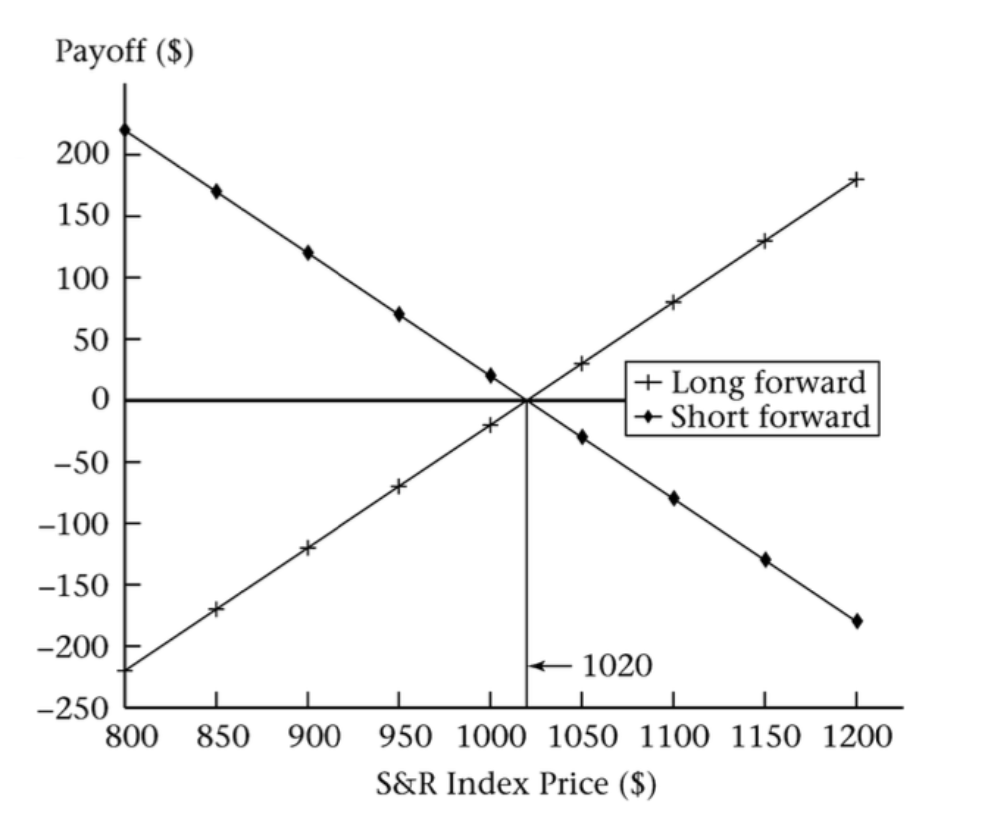
\includegraphics[scale=0.4]{images/forwards.png} 
\end{center}
\end{itemize}
Some additional considerations when looking at forward contracts include the following:
\begin{itemize}
\item Type of Settlement
\begin{itemize}
\item \underline{Cash}: Less costly and more practical
\item \underline{Physical Delivery}: Often avoided due to significant costs
\end{itemize}
\item Credit Risk of Counter Party
\begin{itemize}
\item Major issue for overt the counter contracts (\textit{credit check, collateral, bank letter of credit})
\item Less severe for exchange traded contracts (\textit{exchange guarantees transactions, requires collateral})
\end{itemize}
\end{itemize}

\subsection{Options}
Some key terms relating to options:
\begin{itemize}
\item \textbf{Call Option}: A non-binding agreement giving the right to buy an asset in the future at a price set today.  This preserves the upside potential while eliminating unpleasant downside for buyer. The seller must deliver if asked.
\item \textbf{Put Option}: A non-binding agreement giving the right to sell an asset in the future at a price set today.  The seller must buy if asked.
\item \textbf{Strike Price}: The amount paid by the option buyer for the asset if they decide to exercise.
\item \textbf{Expiration}: The date by which the option must be exercised or will become worthless
\item \textbf{Exercise Style}: Specifies when the option can be exercised
\begin{itemize}
\item \underline{European}: Can only be exercised on the expiration date
\item \underline{American}: Can be exercised any time before expiration date
\item \underline{Bermudan}: Can be exercised on specific dates
\end{itemize}
\item \textbf{Payoff}: Cash value of a position at any point in time
\item \textbf{Profit}: Payoff minus the future value of the investment in the position
\end{itemize}
The table below summarizes the maximum loss or gain for positions in a forward, call, and put:
\begin{center}
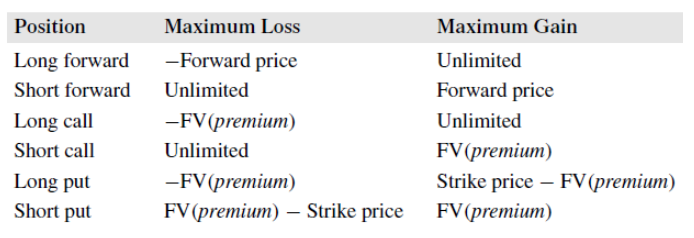
\includegraphics[scale=1]{images/table.png}
\end{center}

\subsection{Embedded Derivatives}
\begin{itemize}
\item A \textbf{Certificate of Deposit} (CD) is an interest-bearing bank account, similar to a note or a bond
\item Banks sell CDs to make money and attract long term stable no-interest bearing deposits
\item To hedge their exposure to CDs, banks purchase call options from a dealer to offset its exposure to short options.
\end{itemize}
\pagebreak


\section{Financial Forwards and Futures}
\hrule \vspace{15pt}
\subsection{Alternative Ways to Stock}
\begin{itemize}
\item \textbf{Outright Purchase}: Ordinary purchase
\item \textbf{Fully Leveraged Purchase}: Investor borrows the full amount
\item \textbf{Prepaid Forward Contract}: Pay today, receive the share later
\item \textbf{Forward Contract}: Agree on price now, pay / receive later
\end{itemize}

\subsection{Pricing Prepaid Forwards}
The term \textbf{prepaid forward} is used to describe arrangements in which a party repays a loan with a predetermined number of shares of stock. If we can price the prepaid forward ($F^P$), then we can calculate the price of $F$.
$$ F = \text{Future Value of } F^P $$
There are 3 methods to price prepaid forwards (with \textbf{no dividends}):
\begin{itemize}
\item \textbf{Pricing by Analogy}: Price $F^P$ of the prepaid forward is the same as the current stock price.  In absence of dividends, delivery timing is irrelevant. $$ F^P_{0,T} = S_0$$
\item \textbf{Pricing by Discounted Present Value of Expected Stock Price:}
$$ F^P_{0,T} = E_0 (S_T)e^{-\alpha T} = S_0 e^{\alpha T} e^{- \alpha T} = S_0$$
\item \textbf{Pricing by Arbitrage:} An arbitrage occurs when one can generate positive cash flows by simultaneously buying and selling related assets with no net investment and no risk.  Derivatives should be priced such that arbitrages are not possible. At equilibrium we expect:
$$ F_{0,T}^P = S_0$$
\end{itemize}
When there are derivatives,  $ F_{0,T}^P = S_0$ is no longer valid, so the pricing changes as follows: 
\begin{itemize}
\item \textbf{Discrete Derivatives}: $D_{t_i}$ at times $i = 1, 2, \cdots n$: $$F_{0,T}^P = S_0 - \sum_{i=1}^n PV_{0,t_i} D_{t_i}$$
\item \textbf{Continuous Derivatives}: With an annualized yield $\delta$:
$$F_{0,T}^P = S_0e^{-\delta T}$$
\end{itemize} 
\pagebreak
\subsection{Pricing Forwards on Stock}
The \textbf{forward price } is the future value of the prepaid forward: $F_{0,T} = FV(F^P_{0,T})$
\begin{itemize}
\item \textbf{No Dividends:} $ F_{0,T}^P = S_0 e^{r T}$
\item \textbf{Discrete Dividends: } $F_{0,T}^P = S_0e^{rT} - \sum_{i=1}^n e^{r(T-t_i)} D_{t_i}$
\item \textbf{Continuous Dividends:} $ F_{0,T}^P = S_0 e^{r - \delta}$
\end{itemize}

\subsection{Creating Synthetic Forwards}
We can offset the risk of a forward by creating a synthetic forward to offset a position in the actual forward contract. This leads to the following:
\begin{itemize}
\item $Forward = Stock - Zero \; Coupon \; Bond$ (buy stock and borrow)
\item $Stock = Forward + Zero \; Coupon \; Bond$ (long forward and lend)
\item $Zero \; Coupon \; Bond = Stock - Forward + $ (buy stock and short forward)
\end{itemize}
\subsection{Futures Contracts}


\pagebreak
\section{Binomial Asset Pricing Model}
\section{Lognormal Stock Price Model}
\section{Black-Scholes Formula}
\section{Exotic Options}
\section{Interest Rate Derivatives}


\end{document}
